\documentclass[10pt,twocolumn]{article}
\usepackage{style}
\usepackage{flushend}
\externaldocument[][nocite]{InnovationZero-Supplement}[InnovationZero-Supplement.pdf]
\begin{document}
\twocolumn[{
\frontmatter{Research manuscript}
\begin{minipage}{\textwidth}
\small
\noindent\textbf{Abstract.}\quadAutomated discovery often alternates proposals with experiments. Can the
consequences of earlier experiments improve the first algorithm proposed for
a new problem, before that algorithm is tested? We define
\emph{InnovationZero} as a data-to-algorithm protocol: a frozen generator
receives permitted training data, commits one reusable learning procedure,
and receives no candidate-specific execution feedback before commitment.
Independent compilation, fitting and evaluation follow. An audit of JopeDime
distinguishes executable construction, catalog-constrained neural learning,
four frontier-labelled regression artifacts and exploratory benchmark
evidence. These establish components of the research program, not its central
generalization claim. In particular, a decoder restricted to a finite catalog
cannot establish synthesis outside that catalog. We specify a prospective,
family-separated comparison with selection, retrieval, conditional generation
and strong fixed learners; failures remain in the denominator. Structural,
behavioral and intervention-based novelty tests distinguish a useful new
procedure from a new source file. Because decisions are judged by quantiles,
weighted deviances and downside risk rather than squared error, the objective
is treated as part of the input, with implemented objective-aware selection,
calibration and program ranking as baselines. Finally, compatible token
accounting and symmetric cost amortization separate retained output from
discovery efficiency. The resulting framework asks how much experimental work can move
into training without confusing a promising first proposal with verified
new knowledge.

\end{minipage}
\vspace{9pt}
\begin{minipage}{\textwidth}
\centering
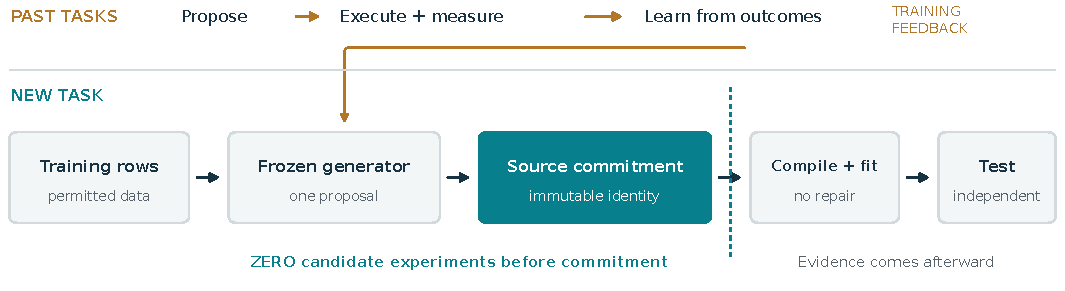
\includegraphics[width=\textwidth]{figures/commitment.pdf}
\captionof{figure}{\textbf{Move experimentation upstream; keep evaluation independent.}
Historical experiments may train the proposer. On a new task, one procedure is committed
before candidate-specific execution or feedback. Compilation, fitting and independent
evaluation follow the commitment. This is the proposed experimental contract, not a
claim that the repository has already demonstrated it.}
\label{fig:commitment}
\end{minipage}
\vspace{10pt}
}]
\thispagestyle{plain}
\section{Can experiments become intuition?}
\label{sec:introduction}

A useful algorithm can arrive before its author knows that it is useful.
This distinction separates proposing an idea from establishing knowledge
about it. Automated discovery systems make the distinction concrete: propose
a program, run an experiment, inspect the outcome, and revise. Their success
raises a second question. After enough experience, can a model make a better
first proposal on a new problem without repeating that experimental loop?

AlphaGo's celebrated Move~37 illustrates both the promise and the boundary.
DeepMind described the move in its second game against Lee Sedol as one its
model assigned roughly a one-in-ten-thousand chance of a human playing.
That estimate characterized a learned prior, not a universal measure of
creativity. The deployed player also searched. AlphaGo Zero subsequently
showed how search-guided self-play could train a strong policy without
human-game supervision; its policy-only and search-assisted evaluations
made the value of the remaining search visible \citep{move37,alphago,alphagozero}.
The important inheritance is the experiment that separates learned
competence from computation performed at the moment of decision.

Algorithm discovery offers an analogous opportunity. AlphaTensor and
AlphaDev use outcome-driven search; FunSearch and AlphaEvolve combine
language-model proposals with executable evaluators
\citep{alphatensor,alphadev,funsearch,alphaevolve}. Learned program synthesis,
library learning and neural symbolic regression already show that experience
can guide or directly supply programs for new inputs
\citep{deepcoder,dreamcoder,symbolicregression}. We therefore make no claim
that data-to-program learning, compositional representations, or the
amortization of search are new in themselves. The question here is narrower:
\emph{what useful algorithmic competence transfers to unseen dataset
families before any candidate-specific experimental feedback is available?}

We study reusable regression learning procedures. The input is a permitted
training table. The output is an executable procedure with fitting and
prediction interfaces, rather than a prediction vector or a set of fitted
coefficients. The generator makes one proposal and commits it before any
candidate execution. Compilation, ordinary estimator fitting and independent
testing then determine whether the procedure works. We call this setting
\emph{InnovationZero}; ``Zero'' describes the pre-commitment feedback budget,
not the amount of training, computation or scientific verification.

This paper is a protocol and evidence audit. JopeDime provides a substantial
implementation and historical evidence base, including constrained program
construction, learned catalog selection and frontier-authored Rust
regressors \citep{jope,clover}. Those pieces must not be assembled rhetorically
into a result they have not jointly demonstrated. The current audit does not
establish a prospective, structurally novel, first-proposal advantage on
untouched families. It identifies the evidence and controls that would make
such a claim meaningful, including outcomes that would falsify it.

Our contributions are fourfold. First, we define an operational commitment
boundary that separates proposal from evaluation. Second, we reconcile
model lineages and exploratory evidence, including a simple support argument
that distinguishes catalog selection from synthesis. Third, we specify a
failure-inclusive, family-level evaluation of predictive utility, novelty
and transfer from experimental history. Fourth, we separate token retention,
artifact throughput and amortized deployment cost. The archived challenge,
complete source submissions and provenance accompany the manuscript in a
separate source volume.

The ambition is a future \emph{Move42}: a useful procedure whose distinctive
mechanism survives independent scrutiny and changes how a problem is solved.
Move42 is our proposed milestone, not AlphaGo's historical Move~37 and not a
discovery reported here. Can a history of experiments improve the first idea
enough to reach it?

\section{The commitment boundary}
\label{sec:setting}

Let a task supply training data $D_{\mathrm{tr}}=(X,y)$ and reserve
$D_{\mathrm{te}}$ for an independent evaluator. The final table column is
always the target. A generator $G_\theta$ maps the permitted training view to
a complete learning procedure $a$, including its configuration and declared
dependencies. After commitment, the evaluator executes
$m=a.\mathrm{fit}(D_{\mathrm{tr}})$ and
$\hat y=m.\mathrm{predict}(X_{\mathrm{te}})$. Test labels never enter the
generator, its encoder, preprocessing, fitting or model selection.
Conditioning on \emph{training} labels is permitted and is not intrinsically
leakage.

\paragraph{One proposal, zero candidate feedback.}
For the primary track the contract is
\begin{equation}
 K=1,\quad E_{\mathrm{pre}}=0,\quad R_{\mathrm{fb}}=0,
 \quad \Delta\theta_{\mathrm{target}}=0.
 \label{eq:zero}
\end{equation}
Here $K$ counts completed candidate proposals; $E_{\mathrm{pre}}$ counts
candidate-specific executions before commitment, including compilation;
$R_{\mathrm{fb}}$ counts feedback-driven repairs or revisions; and the final
term forbids target-specific generator updates. Static constrained decoding
may enforce representation rules, but an executing checker cannot silently
become an extra proposal-selection channel. The decoding rule and seed are
fixed in advance. Multiple sampled candidates, reranking, a rescue fallback
or a replacement after compilation failure belong to a different budgeted
track. A failed first proposal remains a failure.

Commitment freezes source bytes, configuration, generator and encoder
identities, preprocessing contract, random seeds, dependency closure and
resource limits in a content-addressed receipt. A timestamped event trace
records the ordering and evaluator accesses. These are requirements of the
proposed experiment, not claims that the existing runtime already enforces
Equation~\ref{eq:zero}. One autoregressively decoded algorithm can require
many neural forward calls; ``one proposal'' never means ``one forward pass.''

\paragraph{Fitting is a separate computation.}
A committed learner can perform matrix factorization, gradient updates or
boosting during \texttt{fit}. The broad track also permits disclosed
training-only internal validation specified by the frozen algorithm. That
does not send feedback to the generator, but it does perform algorithm
selection inside the learner. We therefore record an orthogonal
\emph{fitting-search} classification. A stricter arm disallows internal
hyperparameter or pipeline search while permitting a predefined optimizer
for the estimator. Historical frontier sources retain their original
behavior and are not relabelled as belonging to this stricter arm.

\paragraph{Universal and conditional generation.}
A universal frontier submission is written once from the challenge and then
fits many datasets. A conditional generator receives a permitted view of
each new dataset before writing its procedure. These are different
information and amortization regimes. Universal submissions are informative
fixed learners, but the primary test of conditioned synthesis requires
matched conditioned baselines. Section~\ref{sec:protocol} specifies both
shared-view and native-view comparisons. An opaque embedding handed to an
unadapted language model is not an adequate information-matched baseline.

\paragraph{Relation to earlier work.}
DeepCoder learns to guide search, DreamCoder learns reusable abstractions,
and AutoML-Zero evolves complete learning algorithms
\citep{deepcoder,dreamcoder,automlzero}. End-to-end symbolic regression predicts
expressions from data, while hypernetworks generate the parameters of other
networks \citep{symbolicregression,hypernetworks}. These are close precedents,
not straw-man alternatives. Our proposed test jointly requires a reusable
learning procedure, an auditable feedback boundary, held-out dataset
families, and a comparison against the same training archive's selectors.
Any incremental claim must survive those controls. A system that learns
excellent selection without structural synthesis should be reported as such.

We use four evidence states: \emph{code-verified} for inspected interfaces;
\emph{repository-reported} for retained historical results not rerun here;
\emph{proposed} for unexecuted experiments; and \emph{unresolved} when the
required artifact is absent. These states apply to claims, not to the
reputation of a model or author.

\section{From experimental history to a first proposal}
\label{sec:method}

InnovationZero is a proposed deployment contract for a \emph{data-to-algorithm}
(D2A) model. Its output is a reusable learning procedure, not a prediction vector
or a set of fitted coefficients. The repository provides components with which
to investigate this contract; the inspected components do not, by themselves,
establish its empirical success. We distinguish their actual interfaces from the
architecture to be evaluated~\citep{jope,clover}.

\subsection{Three existing representations, one proposed interface}

The recorded CLOVER candidate conditions on 2,051 values: 2,048 pooled encoder
values and three query diagnostics. Its PolicyLM is a pre-normalized causal
transformer with 893,957 trainable parameters, width 128, two blocks, four
attention heads, feed-forward width 512, dropout 0.1, and a maximum program
length of 640 representation tokens. A two-layer context projection supplies
the first position; a tied output projection predicts subsequent program tokens.
The end-of-sequence state and context state jointly feed quality, feasibility,
and runtime heads. These representation tokens are not frontier-model language
tokens. The encoder may read the training targets: supervised task conditioning
is permitted, whereas access to outer-test targets is not.

Two other repository interfaces must not be conflated with CLOVER. The Candle
policy consumer accepts a frozen 2,048-value context, assembled as
$512+1{,}024+512$. Hyperion v7 separately produces a 512-dimensional problem
signature. Neither fact establishes a trained 512-dimensional
\texttt{solution\_embedding} or connects such a representation to the historical
CLOVER measurements. The bounded neural-search pipeline also seeds multiple
programs before search. It is not an implementation proof of the one-proposal
contract.

For a permitted training table $D_{\mathrm{tr}}$, with the target in its final
column, and a fixed resource card $b$, the proposed interface is
\begin{align}
 z &= E_\phi(D_{\mathrm{tr}}), &
 s &= H_\theta(z,b), \nonumber\\
 a &\sim P_\theta(\,\cdot\mid s,b), &
 M &= a.\mathrm{fit}(D_{\mathrm{tr}}). \label{eq:d2a-interface}
\end{align}
Here $z$ is the \emph{problem encoding}; $s$ is the learned
\texttt{solution\_embedding}; and $a$ is the complete learning procedure with
\texttt{fit} and \texttt{predict} interfaces. A 512-dimensional $s$ is a proposed
bottleneck to test against direct conditioning and other dimensions, not an
observed property. Source lowering and an immutable commitment to $a$ occur
\emph{before} candidate-specific execution. Fitting $M$, evaluating predictions,
and optionally exporting a fitted deployment artifact occur afterward. Those
outcomes cannot change the committed procedure or trigger a replacement.
One proposal may require many autoregressive neural calls; it is not necessarily
one forward pass.

\subsection{What the protected representation must expose}

The public contract specifies input and output shapes, permitted information,
randomness, resource bounds, supported emission targets, and refusal behavior.
It need not publish the protected grammar or its production rules. Algorithm
decomposition creates structured training objects from procedures: operations,
dependencies, fitted state, and measurable behavior. Such structure can support
learning and comparison without implying that a canonical form decides general
program equivalence. A decomposition study should test whether it improves
transfer beyond retrieval and selection from the same source archive.

The historical CLOVER decoder has finite support: its 6,640-program catalog
contains the only complete programs it can return. Consequently, for this
checkpoint, the probability of generating a program outside that catalog is
zero. This is a support limitation, not an empirical finding about all future
D2A models. A compositional successor must separately establish archive
exclusion, meaningful behavioral differences, and predictive utility.

Typed construction, successful lowering, compilation, bounded execution,
native/emitted agreement, and predictive quality are separate admission stages.
The repository supports Rust, Python, C++17, and JavaScript emission over
qualified subsets; target coverage is not uniform. A refusal is an outcome, not
an invitation to silently try another candidate. Existing parity checks use a
scaled tolerance, $10^{-9}\max(1,|y_{\mathrm{reference}}|)$ per prediction;
they do not certify bitwise equivalence of every program on every input.

\subsection{The training game and its objectives}

At the algorithm level, the decision problem is a one-step contextual bandit:
the context is a training-family problem, the action is a complete procedure,
and the consequence is its measured performance. Autoregressive construction
does not introduce intermediate environmental rewards. \emph{Algorithmic
self-play} can describe repeated training against an archive of prior
procedures, provided the archive, comparison identity, update rule, and control
are specified. A moving archive alone does not demonstrate self-improvement.

For two inner folds, let $r_j$ denote candidate RMSE and $b_j$ the RMSE of a
mean predictor fitted on the complementary rows. Historical quality is
\begin{equation}
 q(c,a)=-\frac12\sum_{j=1}^{2}
 \log\frac{\max(r_j,\varepsilon_c)}{\max(b_j,\varepsilon_c)}.
 \label{eq:inner-quality}
\end{equation}
The floor is scale-aware. The regression target clips $q$ to
$[-\log 1000,\log 1000]$; a separate rounded grid defines ties.
These inner-CV labels are training signals, not untouched generalization
estimates. The implemented native objective is
\begin{align}
 L_6={}&L_{\mathrm{CE}}+0.25L_{\mathrm{BT}}+0.10L_{\mathrm{list}}\nonumber\\
       &+0.25L_q+0.10L_{\mathrm{feas}}+0.05L_{\mathrm{rt}}.
 \label{eq:l6}
\end{align}
Every term is averaged within supported contexts, then across those contexts.
Sequence cross-entropy uniformly averages actual eligible teachers; it is not
the quality-weighted teacher loss of a separate generic implementation.
Measured generated programs supervise auxiliary heads and ranking, but do not
automatically become imitation targets in the described v1/v2 objective.
Unknown targets contribute no fabricated value. Appendix~\ref{app:methods}
gives the precise supports and reductions.

Ranking losses train the quality head, not complete-program probabilities
directly. Falling $L_6$ therefore does not establish improved deployed
proposals. Similarly, the historical best-of-eight surplus
$J_8=\mathbb{E}[\max(h_c,q_1,\ldots,q_8)-h_c]$ can improve while the first
proposal deteriorates. InnovationZero instead proposes
\begin{equation}
 J_1(\theta)=\mathbb{E}_{c,a\sim\pi_\theta(\cdot\mid E_\phi(c),b)}[u(c,a)],
 \label{eq:first-proposal-objective}
\end{equation}
with successful outcomes assigned $u=\operatorname{clip}(q,-1,1)$ and qualifying
failures assigned $-1$. This prospective utility is distinct from historical
$q_{\mathrm{opt}}$; raw error and failure counts remain necessary. Training can
compare imitation, preference updates, and an on-policy score-function estimator
of $J_1$ under matched data and compute. None is asserted here to have won.

The recorded optimizer is AdamW, initially $3\times10^{-4}$ with weight decay
0.01, bias/norm exclusions, gradient clipping at 1, and plateau halving toward
$10^{-6}$. A v2 restart retains optimizer moments and adds a 0.2-weighted exact
finite-support KL anchor to frozen v1 on selected training contexts. Restart-only
and equal-compute controls are therefore required. Dataset aliases and variants
inherit their parent-family role; encoder preprocessing and normalization are
fitted using permitted training information. Fresh-family evaluation and
independent post-commitment measurements decide whether experimental history
has improved the first proposal.

\section{What the existing evidence establishes}
\label{sec:evidence}

We distinguish implementations from executed results, and executed results from evidence for the proposed generalization claim. The audit pins \texttt{main} at \texttt{bdf9441a}; the four-artifact comparison is separately pinned to PR~407, commit \texttt{584713e}. These are evidence snapshots, not an assertion that an unmerged branch is part of \texttt{main}. We inspected source and receipts; we did not retrain a model or rerun a predictive benchmark for this publication. The machine-readable claim ledger records full revisions, source paths and hashes~\citep{jope,clover}.

\subsection{Working infrastructure, different claims}
The repository implements program construction, fitting, source emission, benchmark adapters and neural proposal machinery. Those capabilities make the proposed experiment plausible; they do not make its outcome known. A constrained construction can still fail compilation, execution, numerical parity or predictive evaluation. Each is a separate admission outcome, with language and operator-subset coverage recorded explicitly.

The reported CLOVER v1 outcome head attained pairwise accuracy $0.506$ (95\% lineage-bootstrap interval $[0.441,0.568]$) on fresh programs in 32 kept development contexts, compatible with chance. Later offline contextual-surrogate work reported a ranking increase of $0.046$ ($[0.040,0.052]$) across 1,136 frozen shadow contexts from 255 parents. That positive result is post-iteration shadow validation; the repository explicitly retains \texttt{flywheel\_established=false}. Neither observation licenses a universal claim that learned proposal fails or that recursive improvement succeeds. They locate an unresolved transfer problem~\citep{clover}.

The corrected public-development engine ladder reports rank 31 of 304 and Elo 1687.0, with 42/45 dataset coverage. The separately published 2259.8 rank-one row is a test-selected oracle envelope, including minima over 63,108 test-scored evaluations on 42 datasets. It is not a held-out performance result. The same-cut engine comparison reports Elo 1556.6 and rank 3 of 15, but uses ten favourably selected datasets, top-five deepening and 5/10 finalist coverage; its engine searches 32 programs across eight rounds on each cut. These are distinct experiments, none a qualified first-proposal neural evaluation. Elo values from different panels and opponent pools must not be placed on a common performance axis~\citep{jope}.

\subsection{Four frontier-labelled source artifacts}
The archived challenge fixes the target as the final column, exposes a reusable \texttt{fit}/\texttt{predict} contract, and requires safe, standalone Rust. Complete Opus-, Astra-, Sol- and Gemini-labelled source files and provenance are retained in the source appendix. The first three were present on the pinned main revision; the replacement Gemini artifact is from the separately pinned branch. Their source sizes are respectively 66,536, 27,729, 25,011 and 96,694 bytes.

Artifact identity is stronger than authoring attribution. Astra and Sol disclose prior project context, and Sol lacks exact served-model telemetry. The Gemini replacement receipt records an owner-supplied filename, with no authoring-session or exact provider/model revision evidence. These sources therefore remain historical pilots, not interchangeable pristine challenge attempts. Their use of internal validation is also relevant: frozen universal learner code may select settings while fitting. That is compatible with a no-\emph{generator}-feedback contract, but not automatically with the stronger no-algorithm-search track.

\begin{figure}[t]
  \centering
  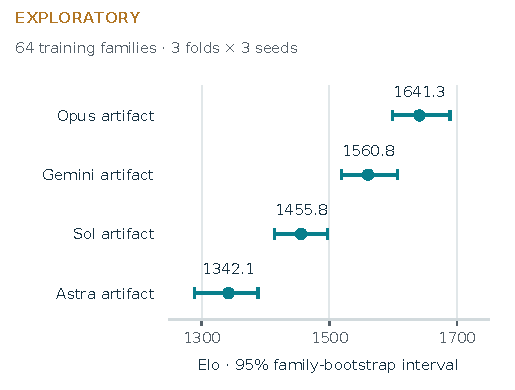
\includegraphics[width=\columnwidth]{figures/elo.pdf}
  \caption{\textbf{Exploratory artifact comparison.} Four-source Elo estimates and 95\% family-bootstrap intervals, redrawn from the pinned result receipt. There is no InnovationZero $K=1$ entrant. The panel contains 64 existing training families and prepared inner-CV contexts; preprocessing and adaptive-history caveats prevent an untouched-family claim. Short labels refer to the exact archived source IDs, not independently authenticated provider revisions.}
  \label{fig:artifact-elo}
\end{figure}

\subsection{Exploratory comparisons, with their limits}
The branch report evaluates 64 families, three folds and three seeds: 576 fitted cells per artifact. The three earlier artifacts' 1,728 fits are reused; 576 Gemini fits are added. All reported cells completed. RMSE is pooled across folds within each family and seed; Elo fits fractional, seed-averaged pairwise outcomes. The reported uncertainty resamples families 10,000 times, keeping repeated seeds together. Figure~\ref{fig:artifact-elo} reproduces the reported estimates without rerunning the fits.

The historical receipt identifies three limits that remain material despite complete coverage: these are current training families; canonical stored preprocessing was fitted before the original train/test split; and seed-41 outcomes were inspected before seeds 73 and 109 were fixed. Some inputs, prediction receipts and analysis programs remain in external custody. Thus, the figure describes these four artifacts on this exploratory panel. It does not establish performance on independent families, compare pristine models, or evaluate the proposed InnovationZero generator.

Ranking frequency and error magnitude answer different questions. Gemini's fractional match score against Sol is $65.625\%$, whereas its majority-family wins are $45/64=70.3125\%$. The oriented geometric-mean error ratio is $\mathrm{RMSE}_{\mathrm{Sol}}/\mathrm{RMSE}_{\mathrm{Gemini}}=0.8468$ (95\% interval $[0.6234,1.0554]$): Gemini's point estimate is about $18.1\%$ higher, not $15\%$. The interval crosses parity, and none of the three reported Gemini comparisons is significant after its stated Holm adjustment. The source appendix preserves original receipts unchanged; this interpretation corrects their compressed prose.

Finally, Gemini's 1,985.8 seconds of aggregate fitting came from a different host than the historical fits. It cannot support a controlled speed ratio. Historical effort report C is linked to Opus by the repository record; report D remains unattributed and is not assigned to Gemini by resemblance of names. These limits motivate the prospective, failure-inclusive protocol rather than diminishing the value of preserving the observations.

\section{A prospective test of first-proposal competence}
\label{sec:protocol}

The central experiment asks whether prior measured outcomes improve the first
useful procedure for a new problem, beyond selecting a complete procedure from
the same archive. The protocol below is a proposed study, not a registered or
completed campaign. Its thresholds specify what stronger claims would require;
they are not results. The available repository evidence motivates these controls
but does not substitute for them \citep{jope,clover}.

\subsection{Commit first; evaluate independently}

For each outer-training context, the primary proposer receives only permitted
training information and a common resource card. It must produce one complete
procedure and commit its source, constants, dependencies, configuration and
component identities before candidate-specific execution or feedback. The
contract is Equation~\ref{eq:zero}: $K=1$, no precommit candidate execution,
no feedback-driven revision and no target-specific generator update. One
autoregressive trajectory may involve many neural forward calls. A deterministic
structural check may refuse an output, but refusal consumes the attempt: neither
resampling nor replacement is allowed. Compilation follows commitment. A compiler
failure therefore remains a failure of the primary attempt; diagnostics cannot
return to the proposer for repair.

An isolated supervisor records event order and source hashes rather than trusting
a model's declaration that it used no feedback. The evaluator subsequently
compiles, fits and scores the unchanged source. The training table's final column
is the target; prediction receives features only. Fitting coefficients, inducing
trees under a fixed rule and other declared parameter optimization are allowed.
Selecting alternative procedures inside \texttt{fit} is disclosed as
fitting-time search, not hidden by the proposal budget. Validation stopping and
configuration selection must be recorded separately. The primary comparison
prespecifies its fitting-search class; the stricter arm excludes configuration
search, while historical learners with CV/HPO retain their fully costed behavior.
Zero proposer feedback is not a claim that fitting performs no computation or
uses no training labels.

\subsection{Independent families and matched information}

The initial planning target is at least \textbf{240 independent confirmation
families}, subject to development-only power simulation. This roster has not
been assembled or evaluated for the proposed study. An additional, disjoint
family lock is required for mechanism confirmation. Real measured regression
tasks should span several domains; multiple stations, targets or derived tables
from one acquisition process must not inflate the independent-family count.
Each registry record binds provenance, rights, target units, transformations,
family membership, prior exposure and exact source/split identities.

Meta-training, validation and confirmation are assigned by family before
candidate generation. Descendants inherit their parent's role. Grouped and
temporal tasks retain appropriate outer splits and information-availability
rules. Imputation, category dictionaries, scaling and encodings are fitted only
on the permitted outer-training rows. Unknown upstream encoder exposure is
reported separately from project-level holdout; a newly downloaded public table
is not proof of pretraining independence.

Conditional methods receive the same deterministic, training-only generation
view: sampled rows, neutral feature identifiers, permitted targets and resource
metadata. The packet and retained dimensions are hashed. Size limits and any
label-independent feature reduction are fixed before scoring; no provider may
silently truncate its input. The native encoder consumes that same view, while
an explicitly separate full-data arm can measure the cost of compression.
Committed learners may fit on the complete outer-training partition. Test labels
remain exclusively with the scorer; test-feature transduction is not part of the
primary information contract.

\subsection{Comparators and the value of experimental history}

Three cohorts answer different questions. A \emph{universal} frontier session
writes one reusable regressor from the neutral challenge alone, paying authoring
cost once. A \emph{conditional} generator receives the common task view and
writes one procedure per context. A \emph{search-assisted} system evaluates
candidates under an explicit target-time budget. Comparing an informed
conditional generator only with an uninformed universal author cannot identify
the effect of architecture or learning.

The primary comparator is the strongest eligible complete-program selector or
nearest-neighbor retriever, chosen on validation and then frozen. Both receive
the same archive and task information as synthesis. Controls include a fixed
ridge learner, current catalog policy, random legal construction, shuffled
context, matched-support imitation, a direct decoder and conditional frontier
generation. A bank distilled from development-time synthesis outputs provides a
stronger portfolio explanation: freeze that bank before confirmation and ask
whether new synthesis still adds value. Practical comparisons include historical
frontier artifacts and strong fixed/tuned tabular learners with declared budgets.
The historical artifacts do not establish pristine fresh-session eligibility.

The decisive secondary study crosses independent training-history levels with
target-candidate evaluation budgets $E\in\{0,1,8,32\}$. At $E=0$, every arm is
strictly $K=1$. Positive budgets permit inner-training evaluation and fixed-rule
selection before an independent outer score, and are explicitly search-assisted.
Outcome-trained models are compared with same-archive retrieval, equal-support
imitation and equal-compute static-data controls. Archive growth, extra updates
and broader construction support must not masquerade as a learning effect.
Multiple training seeds assess replication; the primary checkpoint is chosen
without confirmation outcomes. The resulting quality-versus-search curve is a
planned analysis, not an assumed rising trajectory.

\subsection{Utility, failures and uncertainty}

For family $f$, task $t$ and outer context $r$, let $e_{ftr}$ be the learner's
test RMSE and $b_{ftr}$ that of a training-fitted mean predictor. A positive floor
$\epsilon_{ftr}$ is computed from training targets only. Define
\begin{align}
 q^{\mathrm{te}}_{ftr}&=\log
   \frac{\max(b_{ftr},\epsilon_{ftr})}{\max(e_{ftr},\epsilon_{ftr})},\\
 u_{ftr}&=
 \begin{cases}
 \operatorname{clip}(q^{\mathrm{te}}_{ftr},-1,1),&\text{valid completion},\\
 -1,&\text{method failure}.
 \end{cases}
\end{align}
The evaluator alone computes test errors. Refusal, compile failure, timeout, OOM,
nonfinite predictions, shape errors and protocol violations remain in the
denominator. Infrastructure outages follow a method-blind retry rule using the
same source; they never authorize a new proposal. Raw RMSE, MAE, $R^2$, completion
and failure categories accompany the clipped endpoint.

Average paired utility differences within each family, then weight families
equally. The proposed superiority criterion is a lower two-sided 95\% interval
above \textbf{0.02 utility units} against the locked selector/retriever. This is
not a claim of 2\% RMSE improvement. Paired family resampling retains all tasks,
outer contexts and methods together; folds and bootstrap draws do not increase
the experimental sample size. The primary interval conditions on the frozen
checkpoint; training-seed dispersion is reported separately. Power simulation,
rare-failure bounds, multiplicity and stopping rules are specified in the
supplementary analysis contract. Elo is secondary and panel-dependent; overlapping
rating intervals do not establish noninferiority.

\subsection{Useful structure and the Move42 milestone}

Novelty is assessed against the complete teacher, catalog, retrieval and
representation-training archive, not merely the most recent minibatch. Before
outcome unblinding, reviewers compare anonymized source and documented surface
normalizations. Changes only to names, constants, fitted state, dead code or
compiler expansion do not establish a new reusable structure. General semantic
equivalence is not claimed to be decidable by this audit.

Report the all-attempt intersection of valid, out-of-archive and useful outputs,
with family uncertainty and unresolved judgments counted conservatively. A
predeclared useful-output rule compares error with fixed ridge and the locked
selector under common resource limits. Withheld composition families test a
stronger form of transfer than an unseen source hash. Exact-string rarity under
another generator is not a novelty criterion.

\emph{Move42} names a stronger, future milestone: a qualifying committed source
whose unfamiliar structure contributes useful behavior on reserved families.
A deterministic case-selection rule is frozen first. An intervention removing or
replacing the structure, a matched-complexity control and nearest archive
neighbors are fixed before opening mechanism outcomes. If no case qualifies,
the paper reports no Move42. Independent mechanism confirmation, favorable
economics and repeated self-improvement are separate claims; none follows from
a successful compiler check or an improved average utility alone.

\section{The objective belongs to the problem}
\label{sec:objectives}

Section~\ref{sec:setting} treats a task as a training table. In practice a
task also has a cost of error, and that cost is rarely squared error.
Forecasting theory has held for half a century that the decision loss, not a
convenient norm, defines a good prediction~\citep{granger1969,elliott2008}.
Under squared error the optimal point forecast is the conditional mean; under
an asymmetric linear cost it is the conditional quantile at the cost ratio;
under LinEx it is a shifted mean whose shift depends on the predictive
variance~\citep{varian1975,christoffersen1997}. Gneiting shows that scoring a
point forecast with a function that is inconsistent with the functional the
decision needs can lead to badly misguided conclusions~\citep{gneiting2011}.
Applied fields encode the same lesson. Energy forecasting competitions score
quantiles with the pinball loss~\citep{hong2016gefcom}; retail competitions use
scaled and weighted errors~\citep{makridakis2022m5}; actuaries fit claim
frequency with exposure-weighted Poisson deviance and judge risk ranking with
Gini indices~\citep{frees2011gini}; hydrologists use efficiency criteria such
as KGE~\citep{gupta2009kge}; investment managers penalize downside deviation
rather than volatility~\citep{sortino1994}.

\paragraph{Human design does not follow the objective.}
Learning algorithms are nevertheless designed for a few convenient losses. A
new estimator, with its fitting rule, numerical safeguards, regularization
and tests, is a research and engineering project. Its cost is recovered only
when many users share its objective. General libraries therefore admit custom
objectives through narrow interfaces, typically a per-row loss with a gradient
and Hessian~\citep{xgboost}. Objectives that are non-differentiable, that
aggregate over a sequence (Sortino, maximum drawdown, expected shortfall), or
that read quantities outside the prediction (a unit margin, an exposure, an
imbalance price) fall outside that interface. The usual workaround fits a
squared-error model and then reports the real cost. No organization can ask a
human researcher for a new learning algorithm per cost function; the long tail
of objectives is served by procedures designed for someone else's loss.

\paragraph{Objective-conditioned commitment.}
The InnovationZero boundary extends directly. Let $L$ be a declarative,
content-addressed specification of the evaluation objective. The generator
receives the permitted training view and $L$, and commits
\begin{gather}
 a = G_\theta(D_{\mathrm{tr}}, L), \label{eq:objective}\\
 \hat y_{\mathrm{te}} = a.\mathrm{fit}(D_{\mathrm{tr}}).\mathrm{predict}(X_{\mathrm{te}}),
 \qquad \mathcal{E}_L(a) = L(y_{\mathrm{te}}, \hat y_{\mathrm{te}}). \nonumber
\end{gather}
The objective's identity is frozen with the procedure, and
Equation~\ref{eq:zero} is unchanged: conditioning on $L$ is permitted
information, not feedback. If the generator writes procedures, the marginal
cost of serving a new objective becomes compute rather than researcher time.
The historical frontier-authored regressors of Appendix~\ref{app:effort}
reached source in roughly 11 to 25 minutes of estimated, unmetered authoring
time. None was asked to specialize to a cost function, but the same economics
would make one procedure per objective affordable. That long tail, where no
human would write a dedicated learner, is where an amortized proposer could
differ most from human algorithm design. It is also
a claim that requires the controls below.

\paragraph{What the repository implements.}
The code-verified interface represents $L$ as strict JSON: 38 built-in
objectives with explicit parameters, bounded row expressions over targets,
predictions and declared auxiliary columns, nonnegative row weights, and
positive scaled composites. Every specification has a SHA-256 identity
recorded in selection records, model files and search receipts. Three
mechanisms consume it. First, selection among the fixed native learners uses
held-out $L$ rather than RMSE. Second, a cross-fitted monotone output map,
$\max(\alpha+\beta\hat y,\ \ell)$ with $\beta>0$, is learned on out-of-fold
predictions to minimize $L$; it turns a squared-error forecast into the act
$L$ rewards, such as a quantile, an order quantity or a position size, without
changing the estimator. Third, the program search ranks every candidate program
by held-out $L$, so the structure it selects is chosen for the objective.
Parameter fitting inside a program still uses each head's own estimator loss.
These mechanisms are therefore objective-aware baselines, not the
objective-conditioned generator of Equation~\ref{eq:objective}.

\paragraph{Exploratory evidence.}
A repository-reported benchmark
(\nolinkurl{examples/objectives/real-world}) fits six public tables three ways
on the same training rows and scores the same held-out rows with each table's
objective: RMSE selection among six native learners, selection by the
objective, and selection with the cross-fitted output map
(Table~\ref{tab:objective-evidence}). On four of the six tables the
objective chose the same learner as RMSE, so selection alone did not change
the predictions. The output map reduced held-out loss against RMSE selection
by 63\% for a 10th-percentile wind commitment, 49\% for a 90th-percentile
pollution forecast, 35\% for a 4:1 asymmetric exposure cost and 7\% for
relative valuation error. On a chronological S\&P~500 split, selection by the
after-cost Sortino ratio alone chose a different learner and raised the test
ratio from 0.783 to 1.155, while the map settled on a nearly constant full
position (0.839). On exposure-weighted claim frequency the RMSE-selected
learner predicted non-positive rates for 80 of 6{,}781 held-out policies, so
its Poisson deviance is undefined; selection by the objective chose a learner
with positive rates (deviance 0.789), and the floored output map lowered it to
0.637 ($-19\%$). Ranking written programs by the objective was not
sufficient either. On the ten committed regression datasets, a program search
ranked by 90th-percentile pinball loss, with every program still fitted by
squared error, kept a different program than the RMSE-ranked search on all
ten but lowered sealed-test loss on only four (geometric-mean change
$+4.5\%$).
\begin{table}[t]
\centering
\small
\setlength{\tabcolsep}{4pt}
\caption{Held-out objective values for three arms on six public tables
(single deterministic splits, one seed). Lower is better except Sortino.}
\label{tab:objective-evidence}
\begin{tabular}{@{}llrrr@{}}
\toprule
Table & Objective & RMSE-sel. & Obj.-sel. & + map \\
\midrule
wind & pinball, $\tau=0.1$ & 1.410 & 1.410 & 0.517 \\
houses & MAPE & 0.210 & 0.210 & 0.195 \\
pm10 & pinball, $\tau=0.9$ & 0.240 & 0.240 & 0.122 \\
no2 & asymmetric, 4:1 & 0.975 & 0.975 & 0.629 \\
sp500 & Sortino, net of cost & 0.783 & 1.155 & 0.839 \\
freMTPL & weighted Poisson & undef. & 0.789 & 0.637 \\
\bottomrule
\end{tabular}
\end{table}
These are single splits of
small, public and previously studied tables, with one seed and no family
separation, and they measure a decision layer rather than synthesis. They
show that ranking helps only when some candidate already suits the objective
(two tables of six); otherwise the objective must change what is fitted or
written. They set the baseline an objective-conditioned proposer must beat.

\paragraph{An objective-conditioned protocol.}
The family-level protocol of Section~\ref{sec:protocol} gains an objective
axis. Each confirmation family is paired with objectives drawn from declared
classes: quantile and asymmetric costs, deviances with exposure weights,
relative errors, ranking objectives and sequence-level risk measures. Some
classes are withheld entirely from training. Three comparisons are required.
A cross-objective matrix commits $a_i$ for $L_i$ and scores it under every
$L_j$; an objective-conditioned proposer should win on the diagonal, not
merely on average. The controls are the implemented baselines: an RMSE learner
with cross-fitted calibration for $L_j$, objective-aware selection among the
archive's fixed learners, and the same generator with $L$ withheld. Failures,
including procedures that cannot be scored under $L$, remain in the
denominator. A generator that only reproduces calibration would be reported
as such.

\section{What does an algorithm cost to propose?}
\label{sec:accounting}

Token yield is meaningful only after specifying the object, unit and phase.
Four quantities should remain distinct: retained model output, compiler-qualified
source, expansion from an internal representation, and useful algorithms per
unit resource. A deterministic emitter can retain every printed token while
producing an unhelpful procedure. A 512-coordinate vector is not 512 language-model
tokens, and source expanded from it is not evidence of near-100\% discovery
efficiency.

For directly observable text under one pinned analysis tokenizer, let $S$ be
source spans retained from model output and $O$ all visible output, including
discarded drafts and tool-call text. Let $R$ be additional, nonoverlapping
reasoning tokens and $I$ all processed input in compatible units. Then
\begin{equation}
 Y_{\mathrm{visible}}=\frac{S}{O},\qquad
 Y_{\mathrm{all}}=\frac{S}{I+O+R}.
\end{equation}
The second ratio is unavailable when hidden reasoning cannot be counted in the
same units. Provider-native usage is a parallel ledger, preserving raw overlap
semantics: reasoning may already be included in output total, and cached input
may already be a subset of input total. Neither is added twice. Deduplicated
input content is a separate analysis, not processed or billable usage. Missing
counters remain unknown rather than zero.

For a latent-to-source pipeline, report learned construction decisions and
emitted source bytes or reference tokens separately. Their ratio is an
\emph{expansion factor}, potentially greater than one. Repository lexical source
counts and compile-yield counters retain their own definitions; they are not
frontier model-token measurements \citep{jope}. Count every attempted output,
including refusals and failures, before reporting useful-source yield.

Historical effort records illuminate these distinctions but do not provide a
controlled model ranking. Astra and Sol estimates use attachment-availability
clock proxies and unmetered token ranges. Report C is repository-attributed to
Opus: its later 94k-plus output already includes 27k reasoning, and belongs to
post-freeze admission/integration. The anonymous single-shot report D remains
unresolved; its source dimensions do not match the located Gemini replacement.
The historical-effort supplement preserves these scopes. This paper performs no new
provider metering or source-authoring experiment.

Measure monotonic phase clocks for parse/preprocess, encode, decode, lower,
commit, compile, fit and predict. Report cold and warm latency, concurrency,
hardware, precision, completion and tail latency. Source tokens divided by a
whole authoring session measure artifact delivery, not neural streaming speed.
Timeouts are censored outcomes, not missing slow cases. A cross-provider service
comparison may have unknown hardware; it cannot establish matched-FLOP efficiency.

For $N$ deployments, the economic comparison is
\begin{align}
 C_{\mathrm{IZ}}(N)&=C_{\mathrm{history}}+C_{\mathrm{train}}+N c_{\mathrm{IZ}},\\
 C_{\mathrm{U}}(N)&=C_{\mathrm{author}}+N c_{\mathrm{U}},
\end{align}
where each deployment cost includes encoding or adaptation, compilation/cache,
fitting and prediction as applicable. A conditional frontier author pays
generation per context; a universal source author does not. Charge all attempts,
and disclose unknown upstream pretraining costs symmetrically. A positive
break-even requires matched quality and positive per-deployment savings. The
operational endpoint is therefore complete cost or latency to a useful fitted
predictor, not the amount of code printed per second.

\section{What a positive result would mean}
\label{sec:discussion}

\paragraph{A narrower claim can be more informative.}
If a first-proposal model outperforms selectors using the same archive, the
result would establish a predictive advantage under that comparison. Only
additional archive-exclusion and structural evidence could attribute the
advantage to constructing procedures beyond the stored complete programs.
Mechanism interventions would then test which new structure matters.
These findings would not by themselves establish new
mathematics, general intelligence or scientific autonomy. If retrieval or a
distilled bank matches the model, the evidence instead supports amortized
selection. If additional target evaluations erase the difference, the
advantage is specific to the low-feedback regime. All three outcomes answer
the paper's question more clearly than a single leaderboard rank.

\paragraph{Experimental science remains necessary.}
Socher's Eureka Machine vision combines public knowledge, measurements,
simulation and physical experiments, coordinated by agents. Recursive's
Flint announcement describes iterative automated research, as a company
report rather than an independent demonstration of unrestricted
self-improvement \citep{socher,socherpillars,recursiveflint}. InnovationZero is
complementary: experimentation produces the history from which a useful
proposal policy might learn. It does not replace independent evidence with
a confident first answer. The supplement contextualizes this relationship
and the distinct critiques associated with Jev and LeCun.

\paragraph{Limits of the present evidence.}
The historical frontier sessions were not a pristine, identically metered
experiment. Provider identity, context exposure and accounting precision
vary. The exploratory four-artifact ladder uses development families and
does not contain an InnovationZero first-proposal entrant. It cannot
establish new-family generalization or comparative generator speed.
Independent repeats of the prospective campaign, with openly admissible
datasets, are still required. Publicly accessible data also require a
rights review before redistribution; an internal research-use decision
does not grant publication rights.

\paragraph{Disclosure and reproduction.}
The public assessment boundary includes actual architecture dimensions,
loss support, task separation, resource contracts, emitted algorithms,
failure records and evaluation code. Private representation productions,
token mappings, reversible decomposition examples and compiler internals
are excluded from this manuscript. This restriction is a real limitation:
an external evaluator can inspect outputs and repeat controlled execution
without being able to reproduce training from scratch. Hashes establish
identity, not access or correctness. Any independent-access or escrow
arrangement must be described only after it exists.

\paragraph{Beyond regression.}
Binary classification would require calibration and discriminative metrics;
multiclass learning would require a label-space and proper-loss contract;
time series would require chronological, entity-aware evaluation and
training-only transformations. Optimization would require a feasible
solution and a resource-bounded objective. Recursive improvement would
require interventions on the proposal or learning system itself and
repeated gains against matched restart and replay controls. These are
future tests, not consequences proved by regression infrastructure. The
descriptive family name \emph{data-to-algorithm models} avoids implying
foundation-model breadth before that transfer is demonstrated.

\section{Conclusion}
\label{sec:conclusion}

InnovationZero asks whether experimental history can become a useful first
algorithmic proposal. Its defining boundary is simple: permitted data enter,
one learning procedure is committed, and only then does candidate-specific
execution begin. That boundary makes the claim testable, but does not make
it true. The present repository supplies construction machinery, learned
catalog policies, frontier-authored artifacts and exploratory measurements;
it does not yet supply the prospective synthesis result.

The next decisive evidence is a failure-inclusive comparison on new
families, against selectors and conditional generators with comparable
information, followed by structural and mechanism tests. A positive result
would quantify what training-time experimentation bought. A negative result
would locate the gap between selecting a known procedure and constructing
a useful new one. Move42 remains an open milestone. The experiment may move
upstream; the obligation to test the idea does not disappear.

\bibliographystyle{plainnat}
\bibliography{references}
\end{document}
